\documentclass[12pt]{report}
\usepackage{graphicx}
\usepackage{scribe_MG}
\usepackage{amssymb}
\usepackage{graphicx}
\usepackage[mathscr]{eucal}
\usepackage[english]{babel}
\usepackage[utf8]{inputenc}  %encodage du fichier
\usepackage[T1]{fontenc}
\usepackage{graphicx}
\usepackage{placeins} 
\usepackage{amsmath}
\usepackage{bbm}

%\newcommand\independent{\protect\mathpalette{\protect\independenT}{\perp}}
\def\independenT#1#2{\mathrel{\rlap{$#1#2$}\mkern2mu{#1#2}}} 
\def\PP{\mathbb{P}}
\def\EE{\mathbb{E}}
\def\indep{\bot\!\!\!\bot}

\newtheorem{remark}{Remark}[section]
\newtheorem{example}{Example}[section]

\begin{document}
\coursetitle{Information Theory, KL, MV, Exponential families}
\semester{2013/2014}
\lecturer{Guillaume Obozinski} \scribe{Thomas Belhalfaoui, Lénaïc Chizat}
\lecturenumber{5} \lecturedate{October 30th}

\maketitle


\section{Information Theory}
\subsection{Entropy}
We will use the following properties (Jensen Inequality):
\begin{enumerate}
\item if $f:\mathbb{R} \rightarrow \mathbb{R}$ is convex and if $X$ is an integrable random variable :
  $$\mathbb{E}_X(f(X))\geq f(\mathbb{E}_X(X))$$
\item if $f:\mathbb{R} \rightarrow \mathbb{R}$ is strictly convex, we have equality if and only if 
 $X$ is constant a.s.
\end{enumerate}


\begin{definition}[Entropy]
Let $X$ be a random variable taking values in the finite set $\mathcal{X}$. We denote $p(x)=P(X=x)$.\\
In information theory, the quantity
$$I(x)=\log \,\frac{1}{p(x)}$$
can be interpreted as a quantity of information carried by the occurrence of $x$. (This is sometimes called self-information). 
Entropy is defined as the expected amount of information of the random variable.
$$H(X)=E_{p(x)} \left[ I(X)\right]=-\sum_{x\in\mathcal{X}} p(x)\,\log \,p(x)$$
The base of the logarithm is the natural base or 2, the latter being more consistent with bit coding interpretations of entropy. In this course we will use the natural logarithm.
\end{definition}


%%%%%%%%%%%%%%%%%
\subsection{Kullback-Leibler divergence}

\begin{definition} [Kullback Leibler Divergence]
Let $p$ and $q$ be two finite distributions on $\mathcal{X}$.
The Kullback Leibler Divergence between p and q is defined by
$$\begin{aligned}
D(p\parallel q) &= \sum_{x\in\mathcal{X}} p(x)\log  \frac{p(x)}{q(x)} \\
&= \sum_{x\in\mathcal{X}} \frac{p(x)}{q(x)} \left(\log\, \frac{p(x)}{q(x)}\right)q(x)\\
&=E_{X\sim q}\left[\frac{p(X)}{q(X)} \log \frac{p(X)}{q(X)}\right]
\end{aligned}$$
\end{definition}

\begin{danger}
KL Divergence is \emph{not} a distance as it is not symmetric.
\end{danger}

\begin{proposition}
$D(p\parallel q) \geq 0$ and equality holds if and only if $p=q$.
\end{proposition}

\begin{proof}
If there exists $x \in \mathcal{X}$ such that $q(x)=0$ and $p(x)\neq 0$ then $D(p\parallel q) =+\infty$. Otherwise, we can without loss of generality assume that $q(x)>0$ everywhere. We make this assumption in the rest of the proof.
By convexity of the function $y \mapsto y \log y$, and by Jensen's inequality, we have
$$D(p\parallel q) =  E_{q} \left[ \frac{p(X)}{q(X)} \log  \left(\frac{p(X)}{q(X)}\right) \right] \geq E_{q} \left[\frac{p(X)}{q(X)}\right]  \log E_{q} \left[\frac{p(X)}{q(X)}\right] =  0$$
since
$$ E_{q} \left[\frac{p(X)}{q(X)}\right]= \sum_{x\in\mathcal{X}} \frac{p(x)}{q(x)}q(x) = \sum_{x\in\mathcal{X}} p(x) =1.$$
Furthermore, $D(p\parallel q)=0$ iff there is an equality in Jensen's inequality above which implies that $p(x)=cq(x)$ $q$-a.s., but summing this last equality over $x$ implies that $c=1$, which in turn implies that $p=q$.
\end{proof}

\begin{proposition}
We have the following inequalities: 
\begin{enumerate}
\item $H(X) \geq 0$ with equality if $X$ is constant a.s
\item $H(X) \leq \log (Card(\mathcal{X}))$
\end{enumerate}
\end{proposition}

\begin{proof}
Since $p(x)=\PP_p(X=x) \leq 1$ then $-p(x)\log p(x)\geq 0$ which implies that $H(X)\geq 0$ with equality iff $-p(x)\log p(x)=0$ for all $x \in \mathcal{X}$, which proves the first point. 
Then 
$$\begin{aligned}
D(p\parallel q) &=- \sum_{x\in\mathcal{X}} p(x) \log q(x) - (-\sum_{x\in\mathcal{X}} p(x) \log p(x))\\
&=- \sum_{x\in\mathcal{X}} p(x) \log q(x)  -H(X)\\
\end{aligned}$$
We choose $q_0 (x) = \frac{1}{Card(\mathcal{X})}$. Then $H(X) = \log (Card(\mathcal{X}))-D$.
Hence $H(X) \leq log (Card(\mathcal{X}))$.
\end{proof}

\begin{definition}[Mutual information]
Let $X,Y$ be two random variables of joint distribution $p_{X,Y}(x,y) = P(X=x,Y=y)$ and with marginal distributions $p_X(x)=\sum_{y}p_{X,Y}(x,y)$ and $p_Y(y)=\sum_{x}p_{X,Y}(x,y)$.
The mutual information of $X$ and $Y$  is defined by
$$\begin{aligned}
I(X,Y)&=\sum_{x,y} p_{X,Y}(x,y) \log \frac{p_{X,Y}(x,y)}{p_X(x)\,p_Y(y)}\\
&=D(p_{X,Y}\parallel p_Xp_Y)
\end{aligned}$$
\end{definition}

\begin{proposition}
$I(X,Y)= 0 \Leftrightarrow X\indep Y$
\end{proposition}

\begin{proof}
 It directly follows from the fact that $D(p_{X,Y}\parallel p_X\, p_Y)=0$ implies that $p_{X,Y}(x,y)=p_X(x)p_Y(y)$ which is the definition of the independence of $X$ and $Y$.
 \end{proof}

\begin{danger}
Independent $\Rightarrow$ not correlated  {\bf but} not correlated $\nRightarrow$ independence\\
The first implication comes from the fact that if $X\indep Y$ then $E(X,Y) = E(X)E(Y)$ and then $Cov(X,Y) = 0$. \\
Counter-example for the reverse implication: if $\Theta$ is a r.v. following the uniform distribution on $[0,1]$ and we define the random variables $X$ and $Y$ by $X=\sin (2\pi \Theta)$ and $Y=\cos(2\pi \Theta)$ then $X$ and $Y$ are not correlated but dependent.
\end{danger}
\begin{remark}
The reverse is only true for Gaussian random variables.
\end{remark}

\subsection{Relation between minimum Kullback-Leibler divergence  maximum likelihood principle}

\begin{definition}[Empirical distribution]
Let $x_1,...,x_N\in \mathcal{X}$ be N  i.i.d.\ observations of a random variable $X$.\\
The empirical distribution of $X$ derived from this sample is $$\hat{p}(x)=\frac{1}{N} \sum_{n=1}^{N}\delta(x-x_n)$$
Where $\delta$ is the Dirac function, null everywhere except in 0 where it takes the value 1.
\end{definition}

\begin{proposition}
Let $p_{\theta}$ be a parameterized distribution on $\mathcal{X}$.\\
Maximizing the likelihood $p_{\theta}(x)$ is equivalent to minimizing the KL Divergence $D(\hat{p} || p_{\theta})$
\end{proposition}



\begin{proof}
$$\begin{aligned} 
D(\hat{p} || p_{\theta}) &= \sum_{x\in\mathcal{X}} \hat{p}(x) \log  \frac{\hat{p}(x)}{p_{\theta}(x)}\\
&=  - H(\hat{p}) - \sum_{x \in \mathcal{X}} \hat{p}(x)\,\log \,p_{\theta}(x)\\
&=  -H(\hat{p}) - \frac{1}{N}\displaystyle\sum_{x \in \mathcal{X}} \displaystyle\sum_{n = 1}^{N} \delta(x-x_n)\,\log \,p_{\theta}(x)\\
&=  -H(\hat{p}) - \frac{1}{N} \sum_{n = 1}^{N} \log \,p_{\theta}(x_n)
\end{aligned} $$
The second term is equal to the opposite of the log-likelihood $p_{\theta}(x)$. Hence the conclusion.
\end{proof}

\begin{remark}
$p_\theta(x) = 0 \Rightarrow \hat{p}(x) = 0$, but $ \hat{p}(x) = 0 \nRightarrow p_\theta(x) = 0$. So we should not try to compute  $D(p_{\theta} || \hat{p})$, because this would rule out all the values of x that we have not encountered yet (i.e. such that $\hat{p}(x)=0$).
\end{remark}

%%%%%%%%%%%%%%%%%
\subsection{Maximum entropy principle}
The maximum entropy principle is a different principle than the maximum likelihood principle and solves a different kind of problem.
It assumes that we use the data to specify a constraint on the possible distribution we choose.
The idea is to maximize the entropy $H(p)$ under the constraint that $p\in \mathcal{P}(\mathcal{X})$ where $\mathcal{P}(\mathcal{X})$ is a set of possible distribution typically specified from the data.

Let 's consider the following examples
\begin{enumerate}
\item A study on kangaroos estimated that $p=3/4$ of the kangaroos are left-handed and $q=2/3$ drink Foster beer. What is a reasonable estimate of the fraction of kangaroos that are both left-handed and drink Foster beer? The maximum entropy principle can be invoked to choose among all distributions of pairs of binary random variables. In particular, one way to formalize that we want to choose the least specific distribution that satisfies these constraints is to find the
distribution with maximal entropy that satisfies the constraints on the marginals.
If $X$ is the variable "is left-handed" and $Y$ "drinks Foster beer", then the problem is formalized as 
$$\max_{p_{X,Y}} H(p_{X,Y}) \quad \text{s.t.} \quad p_{X,Y}(1,0)+p_{X,Y}(1,1)=p, \quad p_{X,Y}(0,1)+p_{X,Y}(1,1)=q.$$
What is the solution to this problem? (Exercise)
\item Among all distributions on $\{1,\ldots,10\}$ what is the distribution with expected value equal to $2$ which has the largest entropy? (Exercise)
\item It is possible to show that the distribution on $\mathbb{R}$ with fixed mean $\mu$ and fixed variance $\sigma^2$ that has maximal differential entropy is the Gaussian distribution.
\item The principle of maximum entropy is also the principle invoked to construct distribution on angles with fixed mean and variance. It leads to the so-called \emph{wrapped normal distribution}. A related distribution on angle which is also a maximum entropy distribution is the von Mises distribution. 
\end{enumerate}
The maximum entropy principle is used often when working with \emph{contingency tables}.

\subsection{Entropy and KL divergence for continuous random variables}
 
Let $X$ be a continuous random variable taking its values in the continuous space $\mathcal{X}$ and let $p$ be its probability density function. We have the following adapted expressions of entropy and KL Divergence:
\begin{itemize}
	\item Differential entropy:
	$$H_{\text{diff}}(p)=-\int_{ \mathcal{X} }{p(x) \log (p(x)) d\mu (x)}$$
	\item Differential Kullback Leibler Divergence:
	$$\begin{aligned}
D_{\text{diff}}(p\parallel q) &= \int_{ \mathcal{X} }{p(x) \log \frac{p(x)}{q(x)} d\mu(x)}\\
&= E_{X\sim p} \left[ \log \frac{p(X)}{q(X)} \right]
\end{aligned}$$
\end{itemize}

\begin{danger}
In the continuous case, the entropy is not necessarily non-negative.
\end{danger}

\begin{remark}
The definition of $H_{\text{\!diff\,}}(p)$ depends on the reference measure $\mu$. This means that $H_{\text{\!diff\,}}(p)$ does not capture any intrinsic properties of $p$ any more, and loses its "physical interpretation" in terms of quantity of information, at least in an absolute sense. By contrast $D_{\text{\!diff\,}}(p\parallel q)$ does not depend on the choice of the reference measure and has therefore a stronger interpretation. 
\end{remark}

\section{Exponential families}

Let $x_1,...,x_N\in \mathcal{X}$ be $N$ i.i.d.\ observations  of a random variable $X$.

\begin{definition}
A statistic $\Phi$ is just a function of the data: $x \mapsto \Phi(x) = \Phi(x_1, ..., x_N)$
\end{definition}

\begin{definition}[Sufficient statistic (statistique exhaustive in French)]
A function $T:x \mapsto T(x)$ is a sufficient statistic for a model $\mathcal{P}_{\Theta}$ if and only if
$$ \forall \theta \in \Theta, \quad p_{\theta} (x)=h(x)\,  g(T(x);\theta)$$
\end{definition}
Note that in order to estimate $\theta$ from data $x$ using the maximum likelihood principle the information of the statistics $T(x)$ carries all the information that is relevant.

Another way of interpreting what a sufficient statistic is is to take the Bayesian point of view. In Bayesian statistics, the parameter $\theta$ is modelled as a random variable and we then have:
$$p(x,\theta)=p(x\vert \theta) \, p(\theta)=h(x) \, g(T(x);\theta) \, p(\theta),$$
which means that $\theta \indep X \mid T(X)$.
\begin{definition}[Exponential family]
Let $X$ be a random variable on $\mathcal{X}$. An exponential family is a family of distribution of the form
$$ p(x;\theta) \, d\mu (x)= h(x)\exp \left\lbrace b(\theta)^T \phi(x) - \tilde{A}(\theta) \right\rbrace d\mu (x),$$
where 
\begin{itemize}
\item $h(x)$ the ancillary statistic,
\item $h(x)d\mu (x)$ the reference measure (or base measure),
\item $\phi(x)$ the sufficient statistic (also called feature vector),
\item $\theta$ the parameter,
\item $\eta = b(\theta)$ the canonical parameter,
\item \~{A}$(\theta)=A(\eta)$ the log-partition function.
\end{itemize}
\end{definition}

\begin{proposition}
\label{expression of A}
$$A(\eta) = \log  \int_{ \mathcal{X}  } h(x)\exp  \left\lbrace \eta^T \phi(x)\right\rbrace d\mu (x)$$
\end{proposition}

\begin{proof} 
$$ 1 = \int_{ \mathcal{X} } p(x|\eta) d\mu (x) \: = \:  e^{-A(\eta)}\int_{ \mathcal{X}  } h(x)\exp  \left\lbrace \eta^T \phi(x)\right\rbrace d\mu (x) $$
\end{proof}

\begin{definition}[Canonical exponential family]
A canonical exponential family is an exponential family which such that $b(\theta)=\theta=\eta, i.e.$:
$$p(x;\eta)=h(x) \exp(\eta^T \phi(x)-A(\eta))$$
\end{definition}

\begin{definition}[Domain] The domain of an exponential family is defined by:
$$\Omega\: = \left\lbrace \eta \in \mathbb{R}^p \mid A(\eta) < \infty \right\rbrace  $$
\end{definition}

\begin{example}[Multinomial model]
Let $X$ be a random variable on $\mathcal{X}=\{0 ,1\}^K$. $X$ follows a multinomial distribution of parameter $\pi \in [0,1]^K$.
$$\begin{aligned}
p(x;\pi) &= \prod_{k=1}^{K}{\pi_{k}^{x_k}}\\
&=\exp \Big (\sum_{k=1}^{K}{x_k \log \pi_k}\Big )\\
&=\exp \Big (\sum_{k=1}^{K}{x_k \eta_k}\Big )\\
&=\exp(\langle x, \eta \rangle )
\end{aligned}$$
In this expression we easily recognize:
\begin{itemize}
\item $\eta = (\log \pi_1,\log \pi_2, \cdots,\log \pi_K)^T$;
\item $ \phi (x)=x$;
\item $ d\mu (x)$ the counting measure
\item $ h(x) = 1$ the constant function equal to one;
\end{itemize}
But we don't recognize $A(\eta)$. Let us find it using Proposition \ref{expression of A}:
$$\begin{aligned}
A(\eta)&=\log \Big (\sum_{x\in\mathcal{X}}{\exp(\eta^T x)} \Big )\\
&=\log \Big (\sum_{k=1}^{K}{\exp(\eta_k)}\Big )
\end{aligned}$$
$$\begin{aligned}
 p(x;\eta)&=\exp(\eta^T x - A(\eta))\\
&=\exp\left(\sum_{k=1}^{K}{\eta_k x_k} - A(\eta)\right)\\
&=\exp\left(\sum_{k=1}^{K}({\eta_k - A(\eta)})x_k\right)\\
&=\exp \left( \sum_{k=1}^{K} {\log \left(  \frac{\exp \eta _k}{\sum_{k'=1}^{K}{\exp \eta _k}}\right) x_k} \right)
\end{aligned}$$
We see that in the first expression of the likelihood in its exponential form, we did not take into account the fact that $\sum_k {\pi_k}=1$. There was a hidden constraint on $\eta$. Now we have a new expression for $\pi_k$ and no more constraint over the values that $ \eta$ can take:
$$\tilde{\pi}_k = \frac{\exp (\eta _k)}{\sum_{k'}{\exp(\eta_k)}}.$$
\end{example}

\begin{example}[Gaussian distribution $(\mu,\sigma)$ over $\mathbb{R}$]
$$\begin{aligned}
p(x;\mu , \sigma ^2) &= \frac{1}{\sqrt{2\pi\sigma^2}}e^{-\frac{(x-\mu)^2}{2\sigma^2}}\\
 &= \exp \left\lbrace x^2 \left( \frac{-1}{2 \sigma ^2}\right) +x \frac{\mu}{\sigma ^2} - \left[ \frac{\mu^2}{2 \sigma ^2} + \frac{1}{2} \log (2\pi \sigma ^2)\right]  \right\rbrace 
 \end{aligned} $$

\noindent
We recognize an exponential family with:
\begin{itemize}
  \item $\phi(x) = (x ,\: x^2)^T $
  \item $\eta = (\frac{\mu}{\sigma^2}, \: -\frac{1}{2\sigma^2})^T = (\eta_1,\: \eta_2)^T$
  \item $A(\eta) =\frac{1}{2}\log \left( -\frac{2\pi}{2\eta_2}\right)  - \frac{\eta_1^2}{4\eta_2}$
\end{itemize}
$$p(x) =  \exp \left\lbrace \phi(x)^T\eta - A(\eta)\right\rbrace $$
\noindent
on the domain: $\left\lbrace\eta \in \mathbb{R}^2, \eta_2 <0 \right\rbrace $.
\end{example}

\begin{example}
Many other common distributions are exponential families: Binomial law, Poisson law ($\mathcal{X} = \mathbb{N} $), Dirichlet law, Gamma law, exponential law.
\end{example}

\subsection{Link with the graphical models}

\begin{figure}[h]
\begin{center}
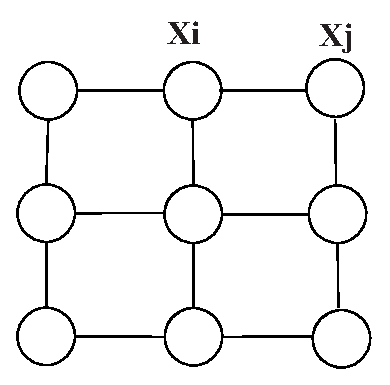
\includegraphics[width = 0.3\textwidth]{modele_ising.eps}
\caption{Ising model}
\end{center}
\end{figure}

\begin{example}[Ising model]

$$\begin{aligned}
p_\eta(x) &= \frac1{Z(\eta)} \exp \sum_{(i, j) \in E} \psi_{ij}(x_i, x_j, \eta)\\
\psi_{ij}(x_i, x_j) & = \rule{0mm}{2pc} V_{ij}^{11} x_i x_j + V_{ij}^{10} x_i (1 - x_j) + V_{ij}^{01} (1 - x_i) x_j + V_{ij}^{00} (1 - x_i) (1 - x_j)\\
\eta &= \rule{0mm}{2pc} (V_{ij}^{kk'})_{\substack{ (i, j) \in E\\ k,\, k' \in \{0, 1\}}}\\
\phi(x) &=\left( \begin{array}{c} x_i x_j\\ (1 - x_i) x_j \\ \vdots \end{array} \right)  _{(i, j) \in E}
\end{aligned}$$

This first expression is overparametrized. We can rewrite the expression with just one parameter per pair $(x_i , x_j)$:
\[ p_\eta(x) = \frac1Z \prod_{(i, j) \in E} \exp \big (\tilde\eta_{ij} x_i x_j \big ) \prod_{i \in V} \exp \big ( \tilde\eta_i x_i\big ). \]
\end{example}

\begin{example}[General discrete graphical model]
In the general case of a discrete graphical model such that $p(x)>x$ for all $x\in\mathcal{X}$, we have:
$$\begin{aligned}
p(x)&= \frac{1}{Z} \prod_{c\in\mathcal{C}}{\Psi_c (x_c)}\\
&=\frac{1}{Z} \exp \left\lbrace \sum_{c\in\mathcal{C}} \log \Psi_c (x_c) \right\rbrace\\
&=\frac{1}{Z} \exp \left\lbrace \sum_{c\in\mathcal{C}} \sum_{y_c \in \mathcal{X}_c} \delta _{\{y_c = x_c\}} \log (\Psi_c (y_c)) \right\rbrace
\end{aligned}$$
Where $\mathcal{X}_c =\{$ set of all possible values of the r.v.\ on the clique $c\}$\\
We recognize:
$$\Phi (x) = \left( \delta_{(x_c = y_c)}\right) _{\substack{ y_c\in\mathcal{X}_c\\ c\in \mathcal{C}}}$$
and
$$\eta = \big( \log (\Psi_c (y_c)) \big ) _{\substack{ y_c\in\mathcal{X}_c\\ c\in \mathcal{C}}}$$
\end{example}

\subsection{Minimal representation}

\begin{remark}
Let $p_\eta(x) = \exp \left(\eta^\top \phi(x) - A(\eta)\right) h(x) d\mu(x)$.\\
The set $\mathcal{N}_\eta:= \{x: p_\eta(x) = 0\} $ actually does not
depend on $\eta$ but only on $h(x)$.
\end{remark}

\begin{definition}[Common set of probability zero]
$$ \mathcal{N} := \lbrace x : h(x)=0 \rbrace $$
\end{definition}

\begin{definition}[Affinely dependent statistics]
We denote $\phi(x) = (\phi_1(x), \ldots, \phi_K(x))^\top$. The sufficient statistics are said to be affinely dependent if:
\[ \exists( c_0, \ldots, c_K ) \neq 0 , \quad \forall x \not\in \mathcal{N}, \; c_0 + c_1 \phi_1(x) + \ldots + c_K \phi_K(x) = 0. \]
\end{definition}

\begin{definition}[Minimal representation of an exponential family]
A vector of sufficient statistics provides a minimal representation of the exponential family these statistics are affinely independent.
\end{definition}

\begin{theorem}
Every exponential family admits at least one minimal representation (not necessarily unique) of unique minimal dimension K.
\end{theorem}

\begin{remark}
We will quite often use redundant (i.e.\ not minimal) representations.
\end{remark}

\subsection{Exponential family of an i.i.d.\ sample}
We consider an i.i.d.\ sample $X_1, \ldots, X_n$ distributed according to $p_\eta$, which belongs to an exponential family. Then
\[ \begin{aligned}
p_\eta(x_1, \ldots, x_n) = \prod_{i=1}^n p_\eta(x_i) = \prod_{i=1}^n  \big [\exp\big (\eta^\top \phi(x_i) - A(\eta)\big ) \, h(x_i)\big ]\\
= \exp \bigg (\eta^\top \Big (\sum_{i = 1}^n \phi(x_i) \Big) - n A(\eta) \bigg ) \: \prod_i h(x_i)
\end{aligned} \]

\begin{enumerate}
  \item The sufficient statistics is $n\bar{\phi}$, where $\bar{\phi}=\frac{1}{n} \sum_{i=1}^{n}\phi(x_i)$,
  \item The canonical parameter $\eta$ and the domain $\Omega = \{\eta \mid A(\eta) < \infty\}$ remain the same as for a single observation,
  \item The log-partition function is $nA(\eta)$.
\end{enumerate}

\subsection{General exponential family}
In general, in an exponential family, we can parametrize $\eta$ with a function $b$ such that  $\eta = b(\theta)$ and $\theta$ in an open connected subset $\Theta$ of $\mathbb{R}^d$.


\begin{definition}[Curved exponential family]
An exponential family is said to be curved if its Jacobian $J=\left\lbrace \frac{\partial b_j(\theta)}{\partial \theta_i} \right\rbrace_{i,j}$ is not full rank.
\end{definition}

\begin{example}
$p_\mu(x) = \mathcal{N}(x; \mu , \mu^2)$
\end{example}


\subsection{Convexity and differentiability in exponential families}

\begin{lemma} [Hölder's inequality]
$$\forall x, y \in \mathbb{R}^d,  \ p, q \geqslant 1 \ \textnormal{such that} \ \frac{1}{p} + \frac{1}{q} = 1$$
\[ |x^\top y| \leqslant {||x||}_p {||y||}_q \quad \textnormal{ where } {||x||}_p = \left(\sum_{k = 1}^n x_k^p\right)^\frac1p. \]

$$\forall f, g: \mathbb{R}^n \rightarrow  \mathbb{R}, \quad
 \int |f(x) g(x)| dx \leqslant \left(\int |f(x)|^p dx\right)^\frac1p \left(\int |g(x)|^q dx\right)^\frac1q. $$
\end{lemma}

\begin{theorem}[Convexity]
In a canonical exponential family, we have the following properties:
\begin{enumerate}
\item $\Omega$ is a convex subset of $ \mathbb{R}^p$
\item $Z: \eta\mapsto \int \exp \left(\eta^\top \phi(x) \right) h(x) dx$ is a convex function
\item $A: \eta \mapsto \log \left(Z(\eta) \right)$ is a convex function
\end{enumerate}
\end{theorem}

\begin{proof}
If $\Omega = \varnothing$ or $\Omega$ is a singleton, the result is trivial.

If not, there exist $ \eta_1,\eta_2 \in \Omega$ such that $\eta_1 \neq \eta_2$. Let $\eta = \alpha \, \eta_1 + (1 - \alpha) \, \eta_2$, \;\; $\alpha \in ]0, 1[$.

\[ \begin{aligned}
\exp(\eta^\top \phi(x)) \: &\leqslant  & &\alpha \exp(\eta_1^\top \phi(x)) &+ &  &(1 - \alpha) & \exp (\eta_2^\top \phi(x))\\
\int \ldots h(x) d\mu(x) \: &\leqslant & &\alpha \int \ldots h(x) d\mu(x) &+ &  &(1 - \alpha) & \int \ldots h(x) d\mu(x)\\
Z(\eta) \: &\leqslant & &\alpha \: Z(\eta_1) &+ & &(1 - \alpha) & \: Z(\eta_2).
\end{aligned} \]
Thus  $Z$ is a convex function. Moreover:
$$\eta_1, \eta_2 \in \Omega \quad \Rightarrow \quad
\ Z(\eta) \leqslant \alpha Z(\eta_1) + (1 - \alpha) Z(\eta_2) < \infty \quad \Rightarrow \quad
\eta \in \Omega$$
which proves that $\Omega$ is a convex set.

\[ \begin{aligned}
Z(\eta) = \int \exp \left( \eta^\top \phi(x) \right) h(x) d\mu(x) = \int \underbrace{(\exp \eta_1^\top \phi(x))^\alpha h(x)^\alpha}_{f(x)^\alpha}   \underbrace{(\exp \eta_2^\top \phi(x))^{1 - \alpha}  h(x)^{1 - \alpha}}_{g(x)^{(1-\alpha)}}   d\mu(x)
\end{aligned} \]

By taking $p = \frac1\alpha$, we obtain:
\[ \begin{aligned}
\int f(x)^\alpha g(x)^{1 - \alpha} d\mu(x) &\leqslant & &\left(\int f(x)^{\alpha p} d\mu(x)\right)^\frac1p  & &\!\!\!\!\!\!\!\!\!\!\left(\int g(x)^{(1 - \alpha) q} d\mu(x)\right)^\frac1q\\
Z(\eta) &\leqslant & &Z(\eta_1) ^\alpha &  &Z(\eta_2)^{1 - \alpha}\\
A(\eta) = \log(Z(\eta)) &\leqslant & &\alpha A(\eta_1) & + &(1 - \alpha) A(\eta_2).
\end{aligned} \]
Hence $A$ is a convex function.
\end{proof}

\begin{corollary}
In a canonical exponential family, the maximum likelihood estimator is the solution of a convex optimization problem.
\end{corollary}
\begin{proof}
The log-likelihood is concave:
\[ \begin{aligned}
\ell(\eta) = \log p_\eta(x) = \eta^\top \bar{\phi}(x) - A(\eta) + \log h(x).
\end{aligned} \]
\end{proof}
\begin{remark}
The theorem does not hold in any of those two cases:
\begin{enumerate}
  \item The family is curved,
  \item $\phi$ is not fully observed and we consider the marginal likelihood of the observations.
\end{enumerate}
\end{remark}

\begin{theorem}
If $\eta \in \overset{\circ}{\Omega} $, then $Z$ is ${\mathcal C}^\infty$ (and so is A) and:

$$ \frac{\partial Z}{\partial \eta_k} =  \mathbb{E}_\eta[\phi_k(x)] Z(\eta) $$

$$ \frac{\partial^m}{\partial \eta_1^{m_1} \ldots \partial \eta_K^{m_K}} Z(\eta) = \mathbb{E}_\eta[\phi_1(x)^{m_1} \ldots \phi_K(x)^{m_K}] Z(\eta) $$

\end{theorem}

\begin{proof}
It is a bit technical but standard to show using the dominated convergence theorem that one can exchange differentiation and expectation in the computations of the differentials of $Z$. One then has
$$
\begin{aligned}
\frac{\partial Z}{\partial \eta_k} & = \int \phi_k(x) \exp \left\lbrace \eta^\top \phi(x) \right\rbrace h(x) d\mu(x)\\
& = \int \phi_k(x) \exp \left\lbrace \eta^\top \phi(x) - A(\eta) \right\rbrace h(x) d\mu(x) \underbrace{exp(A(\eta))}_{Z(\eta)}\\
& = \mathbb{E}_\eta[\phi_k(x)] Z(\eta),
\end{aligned}
$$
which proves the first formula (the general one can be deduced by induction).
\end{proof}

\end{document}
